\subsubsection{Wurfmechanismus}
\begin{figure}[h!]
	\centering
	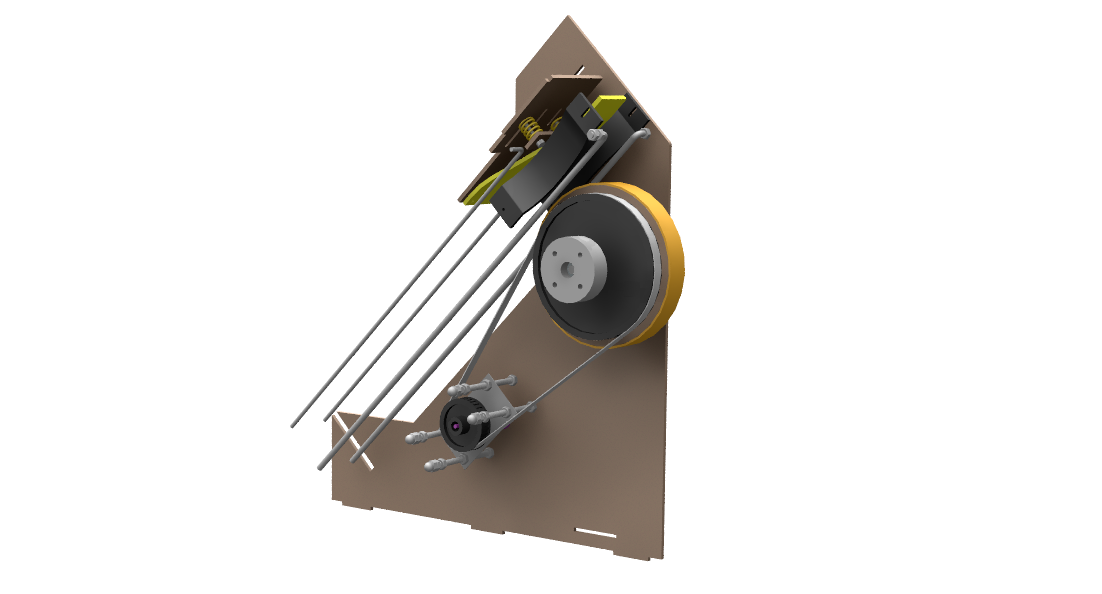
\includegraphics[width=\linewidth]{../../fig/Wurfmechanismus}
	\caption{Wurfmechanismus}
	\label{fig:Wurfmechanismus}
\end{figure}
\paragraph{Komponentenbeschrieb\\}
Hauptstück des Wurfmechanismus ist das Wurfrad, welches durch Drehung um seine eigene Achse die Bälle beschleunigt.
Das aus fünf MDF-Tellern bestehende Wurfrad ist auf einer  Aluminium-Achse montiert. Die Achse ist mit zwei an seinen Enden angebrachten Rillenkugellagern mit den Seitenwänden des Drehturmes verbunden. Auf der Achse befindet sich weiter ein Zahnriemenrad, welches über einen Zahnriemen die Verbindung zum antreibenden BLDC-Motor ermöglicht.
Um die Reibung zwischen den Bällen und dem Wurfrad zu erhöhen, ist ein Gummiband auf das Rad geklebt.

\paragraph{Entwicklungsprozess\\}
Das Wurfrad als beschleunigendes Element hat sich bei vielen anderen Tennisball-Wurfmaschinen bewährt und bot sich daher als sichere Lösung an.
Zu Beginn des Entwicklungsprozesses hielt man es für die beste Lösung ein Rad aus dem Modellbau zu kaufen. Diverse Modellbauräder wurden eruiert. Das Problem bei den Modellbaurädern lag darin, dass diese ein zu geringes Gewicht aufwiesen und zu filigran konstruiert waren. Für unsere Funktion wird ein gewisses Massenträgheitsmoment vorausgesetzt, damit der Beschleunigungsprozess der Tennisbälle einen geringen Einfluss auf die Motorenleistung hat. Darum viel der Entscheid auf eine Eigenkonstruktion des Wurfrades. Mit dieser Lösung, war es möglich, das Rad besser in die Konstruktion einzupassen. Ausserdem konnte es zusammen mit den anderen zu lasernden Komponenten gefertigt werden. Die Halterung des BLDC-Motors ist so konstruiert, dass dieser verschoben werden kann. Dadurch lässt sich die Riemenspannung einstellen.   